%!TEX program = xelatex
% 编译顺序: xelatex -> bibtex -> xelatex -> xelatex
% 国家杰出科学基金申请书正文模板(2024年版)version1.0
% A proposal template for National Natural Science Funds for Distinguished Young Scholar
% 声明:
% 注意!!!非国家自然科学基金委官方模版!!!由个人根据官方MsWord模版制作。本模版的作者尽力使本模版和官方模版生成的PDF文件视觉效果大致一样,然而,并不保证本模版有用,也不对使用本模版造成的任何直接或间接后果负责。 不得将本模版用于商用或获取经济利益。本模版可以自由修改以满足用户自己的需要。但是如果要传播本模版,则只能传播未经修改的版本。使用本模版意味着同意上述声明。
% 强烈建议自己对照官方MsWord模板确认格式和文字是否一致,尤其是蓝字部分。
% 如有问题,可以发邮件到ryanzz@foxmail.com



\documentclass[12pt,UTF8,AutoFakeBold=3,a4paper]{ctexart} %默认小四号字。允许楷体粗体。
\usepackage[english]{babel} %支持混合语言
\usepackage[dvipsnames]{xcolor}
\usepackage{graphicx} 
\usepackage{amsmath} %更多数学符号
%\usepackage{wasysym}
\usepackage[unicode]{hyperref} %提供跳转链接
\usepackage{geometry} %改改尺寸
\usepackage{gbt7714}
\usepackage{natbib}
\setlength{\bibsep}{0.0pt}

%\geometry{left=3.23cm,right=3.23cm,top=2.54cm,bottom=2.54cm}
%latex的页边距比word的视觉效果要大一些,稍微调整一下
%\geometry{left=2.95cm,right=2.95cm,top=2.54cm,bottom=2.54cm}%2020
%\geometry{left=2.95cm,right=2.95cm,top=2.54cm,bottom=2.54cm}
%2024\geometry{left=3.00cm,right=3.07cm,top=2.67cm,bottom=3.27cm}
\geometry{left=3.00cm,right=3.10cm,top=2.67cm,bottom=3.27cm}
\pagestyle{empty}
\setcounter{secnumdepth}{-2} %不让那些section和subsection自带标号,标号格式自己掌握
\definecolor{MsBlue}{RGB}{0,112,192} %Ms Word 的蓝色和latex xcolor包预定义的蓝色不一样。通过屏幕取色得到。
% Renaming floats with babel
\addto\captionsenglish{
    \renewcommand{\contentsname}{目录}
    \renewcommand{\listfigurename}{插图目录}
    \renewcommand{\listtablename}{表格}
    %\renewcommand{\refname}{\sihao 参考文献}
    \renewcommand{\refname}{\sihao \kaishu \leftline{参考文献}} %这几个字默认字号稍大,改成四号字,楷书,居左(默认居中) 根据喜好自行修改,官方模板未作要求
    \renewcommand{\abstractname}{摘要}
    \renewcommand{\indexname}{索引}
    \renewcommand{\tablename}{表}
    \renewcommand{\figurename}{图}
    } %把Figure改成‘图’,reference改成‘参考文献’。如此处理是为了避免和babel包冲突。
%定义字号
\newcommand{\chuhao}{\fontsize{42pt}{\baselineskip}\selectfont}
\newcommand{\xiaochuhao}{\fontsize{36pt}{\baselineskip}\selectfont}
\newcommand{\yihao}{\fontsize{26pt}{\baselineskip}\selectfont}
\newcommand{\erhao}{\fontsize{22pt}{\baselineskip}\selectfont}
\newcommand{\xiaoerhao}{\fontsize{18pt}{\baselineskip}\selectfont}
\newcommand{\sanhao}{\fontsize{16pt}{\baselineskip}\selectfont}
\newcommand{\sihao}{\fontsize{14.2pt}{\baselineskip}\selectfont}
\newcommand{\xiaosihao}{\fontsize{12pt}{\baselineskip}\selectfont}
\newcommand{\wuhao}{\fontsize{10.5pt}{\baselineskip}\selectfont}
\newcommand{\xiaowuhao}{\fontsize{9pt}{\baselineskip}\selectfont}
\newcommand{\liuhao}{\fontsize{7.875pt}{\baselineskip}\selectfont}
\newcommand{\qihao}{\fontsize{5.25pt}{\baselineskip}\selectfont}
%字号对照表
%二号 21pt
%四号 14
%小四 12
%五号 10.5
%设置行距 1.5倍
\renewcommand{\baselinestretch}{1.5}
\XeTeXlinebreaklocale "zh"           % 中文断行

%%%% 正文开始 %%%%
\begin{document}
\begin{center}
{\sanhao \kaishu \bfseries 报告正文}
\end{center}

{\sihao \kaishu {\color{MsBlue} \bfseries (请勿删除或改动下述提纲标题及括号中的文字。)}}
\vskip -5mm
{\color{MsBlue} \subsection{\sihao \kaishu \quad \ (一)主要学术成绩、创新点及其科学意义 \hskip 3mm \textnormal{\kaishu \sihao(建议不超过5000字) }} }
\vskip -3mm
{\color{MsBlue} \kaishu \sihao 着重阐述近5年来在基础研究方面所取得的学术成绩、创新点、研究价值和科学意义等。}

写杰青申请书需要\LaTeX 模板吗?似乎不太有必要。和面上申请书相比,杰青申请书的条目不多,需要公式和文献引用的地方貌似也不太多。但还是制作一个供大家参考吧。


\begin{figure}[!th]
\begin{center}
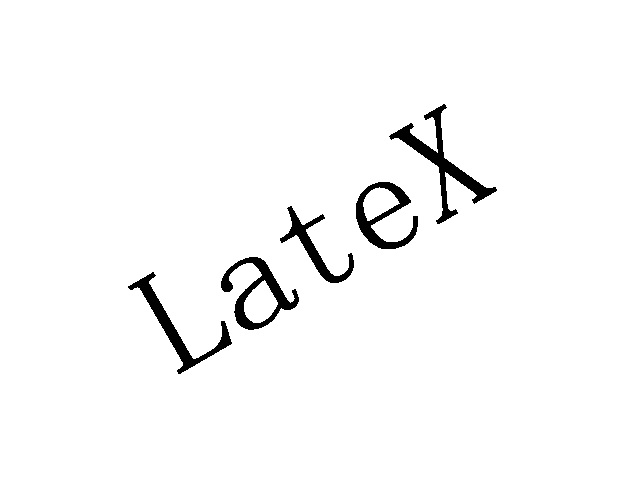
\includegraphics[width=2in]{fig-example.eps}
\caption{{\kaishu 插图可以使用EPS、PNG、JPG等格式。}}
\label{fig:example}
\end{center}
\end{figure}


\vskip 2mm
\subsubsection{1.1 声明}
{\bfseries \color{red} 注意!!!非国家自然科学基金委官方模版!!!}由个人根据官方MsWord模版制作。本模版的作者尽力使本模版和官方模版生成的PDF文件视觉效果大致一样,然而,并不保证本模版有用,也不对使用本模版造成的任何直接或间接后果负责。 不得将本模版用于商用或获取经济利益。本模版可以自由修改以满足用户自己的需要。但是如果要传播本模版,则只能传播未经修改的版本。使用本模版意味着同意上述声明。

祝申请顺利!如有问题,请发送邮件到 \href{mailto:ryanzz@foxmail.com}{ryanzz@foxmail.com}。中了的也欢迎反馈(绝对欢迎!)

\subsubsection{1.2 使用说明}\label{sss:instruction}

\begin{enumerate}
\item 编译环境:在跨平台编译器texlive2022测试可用,编译顺序为: xelatex + bibtex + xelatex(x2)。 windows用户可以用命令行运行批处理文件getpdf.bat,linux用户可以运行runpdf。
\item 本模版力求简单,语句自身说明问题(self explanatory)。几乎只需要修改本tex文件即可满足排版需求。用户掌握最基本的\LaTeX 语句即可操作,其余的可以用搜索引擎较容易地获得。
\item 参考文献采用GB/T 7714 (numerical) 样式以支持中文文献,这样做的另外一个优点是该包兼容natbib,修改参考文献的行距也比较方便,这里也比默认值缩短了一些。
\end{enumerate}

\subsubsection{1.3 图、公式和参考文献的引用示例}
尽管申请杰青不大可能会用到像下面这样简单的公式:
\begin{equation}
\label{eq:ex}
\sqrt[15]{a}=\frac{1}{2},
\end{equation}
我们还是用公式(\ref{eq:ex})举个数学公式的例子。同时,申请杰青也不大可能会用到一个长得很像\LaTeX 的图,但是还是引用一下图\ref{fig:example}。 图\ref{fig:example}并没有告诉我们关于Jinkela\cite{John1997,Smith1900}的任何信息,也没有透露它的产地\cite{Piter1992,grif1998}。尽管如此,最近的研究表明,Jinkela对申请杰青应该没什么作用\cite{John1997}。


%从2023.12.30版本开始,采用GB/T 7714 (numerical) 样式以支持中文文献,这样做的另外一个优点是该包兼容natbib,修改参考文献的行距也比较方便,缩短了一些。如有需要,也可以切换回之前版本用的ieeetrNSFC
%\newpage
%\bibliographystyle{ieeetrNSFC}
\bibliographystyle{gbt7714-numerical}
\bibliography{myexample}
\newpage

{\color{MsBlue} \subsection{\sihao \kaishu \quad \ (二)拟开展的研究工作 \textnormal{\kaishu (建议不超过3000字) }} }
{\color{MsBlue} \kaishu \sihao 着重阐述拟开展的研究工作的创新性构思,主要研究方向和初步研究方案等,请简要阐述。}

申请人如果获得资助,将在以往研究的基础上,继续更新系列模板。

{\color{MsBlue} \subsection{\sihao \kaishu \quad \ (三)其他需要说明的情况 }}

{\sihao \color{MsBlue} \kaishu 1. 申请人同年申请不同类型的国家自然科学基金项目情况(列明同年申请的其他项目的项目类型、项目名称信息,并说明与本项目之间的区别与联系)。}

无。

{\sihao \color{MsBlue} \kaishu 2. 具有高级专业技术职务(职称)的申请人是否存在同年申请或者参与申请国家自然科学基金项目的单位不一致的情况;如存在上述情况,列明所涉及人员的姓名,申请或参与申请的其他项目的项目类型、项目名称、单位名称、上述人员在该项目中是申请人还是参与者,并说明单位不一致原因。}

无。

{\sihao \color{MsBlue} \kaishu 3. 具有高级专业技术职务(职称)的申请人是否存在与正在承担的国家自然科学基金项目的单位不一致的情况;如存在上述情况,列明所涉及人员的姓名,正在承担项目的批准号、项目类型、项目名称、单位名称、起止年月,并说明单位不一致原因。}

无。

{\sihao \color{MsBlue} \kaishu 4. 其他。}

无。
\end{document}


